\documentclass[conference]{IEEEtran}

\usepackage[T1]{fontenc}
\usepackage[utf8]{inputenc}
\usepackage{cite}
\usepackage{amsmath,amssymb}
\usepackage{graphicx}
\usepackage{booktabs}
\usepackage{multirow}
\usepackage{url}
\usepackage{xurl}
\usepackage{hyperref}
\hypersetup{hidelinks}

\title{Labyrinth Breach: A Reproducible Unity ML-Agents Benchmark for Asymmetric Multi-Agent Pursuit-Evasion in Dynamic Mazes}

\author{
\IEEEauthorblockN{
Ahmed Jawed,
Muhammad Sikander Raheem,
Usman Irshad Bhatti
}
\IEEEauthorblockA{
25280017 \quad 25280099 \quad 25280040\\
MS AI, LUMS\\
AI641 -- AI for Robotics
}
}

\begin{document}

\maketitle

\begin{center}
\fbox{\parbox{0.92\linewidth}{\centering\textbf{Superseded course-report version.}
The canonical publication draft is \texttt{paper/labyrinth\_breach\_journal.tex};
results here are retained only for historical comparison.}}
\end{center}

\begin{abstract}
We present Labyrinth Breach, a configurable Unity ML-Agents benchmark for asymmetric multi-agent pursuit-evasion in dynamic maze environments. Three Sentinel agents cooperatively pursue two Runner agents across procedurally generated layouts with shifting walls, exit zones, and partial observability. Agents observe through vector states, 360-degree raycasts, and last-known-position memory, and are trained with PPO under a tactical reward-shaping framework designed to reduce free-rider collapse, cluster convergence, and passive evasion. Beyond the environment itself, we contribute an auditable evaluation pipeline that routes raw Unity logs into run-scoped artifacts, computes outcome and coordination metrics, and supports multi-seed seen/unseen layout evaluation and ablation studies. Preliminary legacy runs suggest that curriculum training improves behavior as environments progress from open arenas to dynamic mazes, but publication-grade claims require the stricter multi-seed protocol described in this paper. The source code and trained models are publicly available.\footnote{\url{https://github.com/ahmedjawedaj/labyrinth-breach-marl}} A demonstration video of trained agents in the dynamic maze is available online.\footnote{\url{https://drive.google.com/file/d/1sxzKtpvVNh_UYYxchMTZzzZNKLDyh09w/view}}
\end{abstract}

\begin{IEEEkeywords}
Multi-agent reinforcement learning, pursuit-evasion, dynamic maze, reward shaping, Unity ML-Agents, PPO
\end{IEEEkeywords}

% ============================================================
\section{Introduction}
% ============================================================

Pursuit-evasion is a classical problem in robotics and multi-agent decision-making. One side attempts to capture while the other attempts to escape. The problem is a natural fit for reinforcement learning (RL) because the desired behavior is difficult to hand-code when the environment involves adversarial interaction, obstacles, partial information, and multiple cooperating agents.

The original course project requires RL-based multi-agent pursuit-evasion using Unity ML-Agents. We extend this requirement into a structured environment called \textit{Labyrinth Breach}, where three Sentinels pursue two Runners inside a maze with exit zones and dynamic topology changes.

Simple chase environments do not capture the full difficulty of multi-agent coordination. In a richer maze setting, effective Sentinel behavior includes trapping, pincer movement, corridor denial, exit blocking, and route cutting. On the other side, effective Runner behavior includes distance management, path selection, survival, and escape through exits. These requirements align the project with robotics-style navigation and coordination problems rather than only direct-motion pursuit.

Our contributions are as follows:
\begin{itemize}
    \item A configurable asymmetric 3v2 pursuit-evasion environment with procedurally generated static and dynamic maze layouts.
    \item A tactical reward shaping framework (\texttt{v5\_active\_agents}) that targets free-rider collapse, clustering, and passive evasion through configurable shaping terms.
    \item A memory-augmented partial observation design combining 360-degree raycasts with last-known-position tracking.
    \item A three-phase curriculum learning pipeline (open arena $\to$ static maze $\to$ dynamic maze) with transfer learning between stages.
    \item A reproducible evaluation and evidence pipeline for multi-seed seen/unseen testing, coordination metrics, and ablations over memory, tactical rewards, dynamic walls, curriculum, and action assistance.
\end{itemize}

% ============================================================
\section{Related Work}
% ============================================================

We organize the related work into four themes that directly support different aspects of our system design.

\subsection{Pursuit-Evasion as a Multi-Agent Problem}

Direct pursuit-evasion papers share the same capture-versus-escape structure as our task. In harder settings, useful behaviors go beyond direct motion and include route blocking, coordinated pressure, spatial entrapment, and strategic escape timing \cite{verma2019mapel,viper2025,gonultas2024,yan2019uncertain,liu2024uav}. Recent work has also shown that coordinated pursuit strategies can emerge naturally from simple reward signals when the environment contains enough structure \cite{haeri2022emergent}. Our environment targets exactly these richer behaviors through maze topology and exit-based objectives.

\subsection{Cooperative and Mixed MARL}

Multi-agent reinforcement learning faces a non-stationarity challenge because all agents update simultaneously. MADDPG addressed this through centralized training with decentralized execution \cite{lowe2017maddpg}. More recently, Yu et al. showed that PPO-based methods serve as strong practical baselines in cooperative settings when tuned carefully \cite{yu2022mappo}. We adopt PPO with parameter sharing as our primary training method because Unity ML-Agents supports it natively and provides a reproducible baseline; stronger centralized-credit baselines such as MA-POCA or MAPPO remain important comparison points for publication-grade evaluation.

\subsection{Credit Assignment}

When multiple agents cooperate under team-level objectives, one agent may contribute by blocking a route or creating pressure while another gets the final capture. Plain shared reward can be too coarse for learning such indirect contributions \cite{rashid2018qmix,foerster2018coma,wang2020implicit,chen2023explicit}. We address this through tactical reward shaping that provides per-agent bonuses for coordination events such as pincer formations and corridor control.

\subsection{Partial Observability}

Pursuit-evasion becomes more meaningful when sensing is limited. With full global state, the task is easier and less realistic. Works on visibility-constrained pursuit-evasion show that line-of-sight, uncertainty, and memory fundamentally change the problem \cite{viper2025,gonultas2024,matrixworld2023}. Our observation pipeline uses vector states combined with ray-based visibility and last-known-position memory rather than global state or camera images.

% ============================================================
\section{Problem Formulation}
% ============================================================

We model the environment as a Partially Observable Stochastic Game (POSG) defined by the tuple $\langle N, \mathcal{S}, \{A_i\}, \{O_i\}, T, \{R_i\}, \gamma \rangle$ where $N{=}5$ agents (3 Sentinels, 2 Runners), $\mathcal{S}$ is the joint state space covering agent positions, velocities, maze configuration, and wall states, $A_i \in \mathbb{R}^2$ are continuous actions for each agent (horizontal and forward movement), $O_i$ is the partial observation function (117 floats for Sentinels, 129 for Runners), $T$ is the transition function governed by Unity physics, $R_i$ is the team-conditioned reward function combining team-level terminal outcomes with role-specific shaping terms (Table~\ref{tab:rewards}), and $\gamma{=}0.99$ is the discount factor.

The Sentinel team wins when both Runners are captured before timeout. The Runner side wins when at least one Runner reaches an exit zone or when the episode times out at 120 seconds (5,000 decision steps). Each episode also features dynamic wall shifts at configurable intervals, changing the maze topology during play.

This formulation supports the study of asymmetric team interaction, coordinated pursuit, tactical escape behavior, partial observability, dynamic environment changes, and generalization to unseen layouts.

% ============================================================
\section{System Design}
% ============================================================

\subsection{Environment Structure}

The implementation includes four scenes of increasing complexity:
\begin{itemize}
    \item \textbf{Open arena baseline:} flat arena with no walls.
    \item \textbf{Static maze:} fixed procedurally generated corridors.
    \item \textbf{Dynamic maze:} walls shift at configurable intervals during episodes.
    \item \textbf{Unseen evaluation maze:} novel layouts not encountered during training.
\end{itemize}

The dynamic maze is the core environment. Walls are generated procedurally from a seed and can shift during the episode by raising or lowering wall pillars on a timer. This prevents memorization of fixed routes and creates trapping opportunities and escape adaptations in real time. Exit zones are placed explicitly for the Runner side, making evasion a goal-directed navigation task rather than pure survival.

\subsection{Agent Architecture}

The codebase separates agent logic, environment control, reward computation, sensing, and logging into distinct modules. \texttt{BaseAgent} handles movement, observation collection, and ML-Agents integration. \texttt{SentinelAgent} extends it with capture-radius logic and target tracking. \texttt{RunnerAgent} extends it with escape and captured-state management. The central \texttt{PursuitEvasionEnvController} manages episode lifecycle, capture detection, reward triggering, and terminal conditions.

\subsection{Observation Design}

The observation pipeline is state-based rather than camera-based. Table~\ref{tab:state_action} shows the complete breakdown. Each agent receives a flat vector containing self-state (position, velocity, heading, alive flag), environment context (time remaining, nearest exit distance and direction, wall proximity, wall shift timer), 360-degree raycasts, last-known-position memory for targets that have left line of sight, and a summary of the two nearest opponents including their relative position, visibility, and threat pressure.

Sentinels cast 14 rays while Runners cast 16 rays. Each ray produces 6 floats: normalized hit distance and one-hot indicators for wall, exit, teammate, opponent, and other object types. This gives Runners wider sensing coverage because their survival depends on detecting threats from all directions.

\begin{table}[t]
\centering
\caption{Observation and action space per agent role.}
\label{tab:state_action}
\begin{tabular}{lcc}
\toprule
Component & Sentinel & Runner \\
\midrule
Self state & 10 & 10 \\
Environment context & 7 & 7 \\
Ray perception (6 per ray) & 84 (14 rays) & 96 (16 rays) \\
Last-known-position memory & 6 & 6 \\
Opponent summary (2 nearest) & 10 & 10 \\
\midrule
\textbf{Total observation size} & \textbf{117} & \textbf{129} \\
\midrule
Action space & 2 continuous & 2 continuous \\
\bottomrule
\end{tabular}
\end{table}

\subsection{Reward Design}

The reward system uses the \texttt{v5\_active\_agents} configuration, which was iteratively developed to address three behavioral failure modes observed during training: (1)~free-rider collapse, where one Sentinel learns to capture while others idle; (2)~cluster convergence, where all Sentinels chase the same Runner in a single file; and (3)~passive evasion, where Runners survive by standing still rather than actively seeking exits.

The reward function combines terminal win/loss signals with distance-based shaping for pursuit and evasion, anti-clustering penalties, idle penalties, exit-seeking shaping, and a tactical coordination layer that rewards events detected by a dedicated \texttt{TrapEventDetector} module. The tactical layer rewards pincer formations, corridor control, exit denial, and dead-end forcing. All weights are loaded from YAML configuration files at runtime. Table~\ref{tab:rewards} lists the final reward weights.

\begin{table}[t]
\centering
\caption{Reward weights (\texttt{v5\_active\_agents} configuration).}
\label{tab:rewards}
\begin{tabular}{lc}
\toprule
\textbf{Sentinel Rewards} & Weight \\
\midrule
Team full capture (win) & $+1.0$ \\
Timeout or escape (loss) & $-1.0$ \\
Individual capture bonus & $+0.25$ \\
Chase progress (per step) & $+0.004$ \\
Chase regression & $-0.003$ \\
Cluster penalty & $-0.015$ \\
Idle penalty & $-0.002$ \\
Wall loop penalty & $-0.002$ \\
Exploration visit bonus & $+0.001$ \\
Orbit stall penalty & $-0.003$ \\
\midrule
\textbf{Runner Rewards} & Weight \\
\midrule
Team exit success (win) & $+1.0$ \\
Both captured (loss) & $-1.0$ \\
Tagged individually & $-0.2$ \\
Survival step bonus & $+0.0001$ \\
Exit approach bonus & $+0.005$ \\
Exit approach regression & $-0.002$ \\
Evade progress & $+0.001$ \\
Threat approach penalty & $-0.002$ \\
Wall loop penalty & $-0.001$ \\
Exploration visit bonus & $+0.001$ \\
Orbit stall penalty & $-0.003$ \\
\bottomrule
\end{tabular}
\end{table}

\subsection{Logging and Reproducibility}

Each training and evaluation run produces four CSV artifacts under a run-specific directory: \texttt{episode\_log.csv} (per-episode outcomes and totals), \texttt{agent\_step\_log.csv} (per-step positions, actions, and distances), \texttt{reward\_audit.csv} (per-event reward attribution by agent, category, and magnitude), and \texttt{replay\_events.csv} (timestamped capture, escape, wall-shift, and tactical events). This structure ties every reported metric back to raw per-step evidence.

% ============================================================
\section{Training and Evaluation Setup}
% ============================================================

\subsection{Training Algorithm}

We train both behaviors with PPO using parameter sharing within each team. All three Sentinels share a single policy network, and both Runners share a separate one. Table~\ref{tab:hyperparams} lists the hyperparameters. The learning rate follows a linear decay schedule over the training run. MA-POCA is supported in the configuration for future credit-assignment experiments but was not used in the results reported here.

\begin{table}[t]
\centering
\caption{PPO hyperparameters (shared by both behaviors).}
\label{tab:hyperparams}
\begin{tabular}{lcc}
\toprule
Parameter & Static Maze & Dynamic Maze \\
\midrule
Learning rate & $3.0{\times}10^{-4}$ & $2.5{\times}10^{-4}$ \\
Batch size & 2048 & 2048 \\
Buffer size & 20480 & 40960 \\
Entropy ($\beta$) & $5.0{\times}10^{-3}$ & $4.0{\times}10^{-3}$ \\
Clip range ($\epsilon$) & 0.2 & 0.2 \\
GAE $\lambda$ & 0.95 & 0.95 \\
Discount ($\gamma$) & 0.99 & 0.99 \\
Epochs per update & 3 & 4 \\
Hidden units & 256 & 256 \\
Hidden layers & 2 & 2 \\
Time horizon & 128 & 160 \\
Sentinel max steps & 1{,}000{,}000 & 1{,}500{,}000 \\
Runner max steps & 1{,}000{,}000 & 1{,}000{,}000 \\
\bottomrule
\end{tabular}
\end{table}

\subsection{Curriculum and Transfer Learning}

Training follows a three-phase curriculum with transfer learning between stages, motivated by evidence that staged difficulty helps agents discover coordination skills that are hard to learn from sparse reward alone \cite{zhang2023curriculum}. Each phase uses \texttt{--initialize-from} to bootstrap the policy network from the previous stage's checkpoint, preserving learned pursuit and evasion skills while adapting to increased environmental complexity. Critically, the network architecture (256 hidden units, 2 layers) is kept identical across all phases to enable seamless weight transfer.

Table~\ref{tab:curriculum} shows the progression. Phase~1 establishes basic pursuit-evasion in an open arena. Phase~2 introduces fixed maze walls, forcing agents to learn spatial navigation. Phase~3 adds dynamic wall shifts, requiring adaptation to changing topology.

\begin{table}[t]
\centering
\caption{Three-phase curriculum progression with transfer learning.}
\label{tab:curriculum}
\begin{tabular}{lccc}
\toprule
Phase & Scene & Steps & Transfer From \\
\midrule
1. Open Arena & 01\_Baseline & 500K & -- \\
2. Static Maze & 02\_StaticMaze & 1{,}000K & Phase 1 \\
3. Dynamic Maze & 03\_DynamicMaze & 1{,}500K & Phase 2 \\
\midrule
\textit{Evaluation} & 04\_UnseenMaze & -- & Phase 3 \\
\bottomrule
\end{tabular}
\end{table}

\subsection{Evaluation Protocol}

We evaluate trained policies in inference mode using fixed ONNX checkpoints. The publication protocol uses three policy seeds (42, 101, 202), one seen dynamic-maze split, and at least five held-out unseen layout seeds (101, 202, 303, 404, 505). All evaluation runs use deterministic action selection and must produce run-scoped raw logs: \texttt{episode\_log.csv}, \texttt{agent\_step\_log.csv}, \texttt{reward\_audit.csv}, and \texttt{replay\_events.csv}. A run is excluded from publication tables if any required log, metadata file, or KPI summary is missing.

The evaluation protocol reports outcome metrics (Sentinel win rate, Runner win rate, escape rate, survival time, and capture times), coordination metrics (pincer episode rate, trap frequency, corridor-block events, exit-denial events, Sentinel spread, and Runner separation), path metrics (path efficiency and route-change proxies after wall shifts), and ablation deltas. Because the current environment includes optional action-assist blending in the controller, publication results must include an action-assist-off ablation before attributing coordination purely to learned policies.

% ============================================================
\section{Results}
% ============================================================

This section separates two evidence layers. First, we retain legacy course-project summaries as historical motivation. Second, we report a validated checkpoint diagnostic produced by the run-scoped pipeline in Section~V-C. Neither layer is sufficient for final journal claims because independent policy-seed retraining and the full ablation matrix remain incomplete.

\begin{table}[t]
\centering
\caption{Preliminary per-phase training performance summary from legacy artifacts.}
\label{tab:phase_results}
\begin{tabular}{lccc}
\toprule
Metric & Open+Static & Dynamic & Unseen \\
\midrule
Episodes & 3{,}228 & 2{,}492 & 30 \\
Sentinel win rate & 100.0\% & 66.8\% & 50.0\% \\
Runner win rate & 0.0\% & 33.2\% & 50.0\% \\
Sentinel mean reward & $+3.545$ & $+0.680$ & $+0.257$ \\
Runner mean reward & $-2.407$ & $-0.993$ & $-0.181$ \\
Wall-loop penalty & $-0.009$ & $-0.364$ & $-0.017$ \\
Cluster penalty & $-0.013$ & $-0.518$ & $-0.035$ \\
\bottomrule
\end{tabular}
\end{table}

The preliminary Sentinel win rate follows a curriculum-driven trend: near-perfect capture in the open arena/static maze setting, reduced dominance in the dynamic maze, and a balanced outcome in a small unseen-layout evaluation. We treat this as motivation rather than proof: stronger claims require repeated evaluation across policy seeds and multiple held-out layouts with confidence intervals.

\subsection{Validated Checkpoint Diagnostic}

After correcting standalone scene, rule-config, and reward-config routing, we evaluated the fixed \texttt{v5\_dynamicmaze} checkpoint pair across one seen layout and five held-out layout seeds. Three evaluation seeds were used, but these are not independent training seeds. Each matrix cell ran for 30 wall-clock seconds in deterministic inference mode. The audit accepted all 18 cells, all 108 required raw/KPI artifacts, and every episode-level scene/rule/reward provenance check.

\begin{table}[t]
\centering
\caption{Validated fixed-checkpoint diagnostic. Confidence intervals are 95\% Wilson intervals over completed episodes.}
\label{tab:validated_diagnostic}
\begin{tabular}{lcc}
\toprule
Metric & Seen & Five unseen layouts \\
\midrule
Completed episodes & 12 & 106 \\
Sentinel wins & 9 (75.0\%) & 73 (68.9\%) \\
95\% CI & [46.8, 91.1]\% & [59.5, 76.9]\% \\
Runner wins & 3 (25.0\%) & 33 (31.1\%) \\
Escape rate & 0.0\% & 25.5\% \\
Mean full capture time & 13.33 s & 21.04 s \\
\bottomrule
\end{tabular}
\end{table}

The aggregate result remains Sentinel-favored, but held-out geometry matters: per-layout Sentinel win rate ranges from 33.3\% on seed 505 to 88.2\% on seed 202. This variation is evidence against a layout-invariant performance claim and motivates longer per-layout evaluation with independently trained policy seeds.

\subsection{Reward Curves}

Figure~\ref{fig:reward_curves} shows the per-episode cumulative reward for both teams across all curriculum phases. The green-shaded region corresponds to the open arena and static maze phases, where the Sentinel reward is consistently high ($+3.545$). The orange-shaded region marks the transition to the dynamic maze, where the Sentinel mean reward drops sharply to $+0.680$ as the Runners learn to exploit wall shifts for cover.

\begin{figure}[t]
    \centering
    
\includegraphics[width=0.48\textwidth]{fig_reward_curves.pdf}
    \caption{Per-episode cumulative reward across curriculum phases. The curriculum transition (vertical line) shows the reward shift as maze complexity increases.}
    \label{fig:reward_curves}
\end{figure}

Figure~\ref{fig:reward_breakdown} decomposes the total reward into terminal, shaping, trap-aware, and penalty components. In the legacy run, terminal reward is the largest component, suggesting that shaping did not completely dominate win/loss learning. The publication pipeline verifies this claim by regenerating reward-breakdown tables from raw \texttt{reward\_audit.csv} files for every run.

\begin{figure}[t]
    \centering
    
\includegraphics[width=0.48\textwidth]{fig_reward_breakdown.pdf}
    \caption{Reward component decomposition. Terminal reward dominates; penalties increase with maze complexity.}
    \label{fig:reward_breakdown}
\end{figure}

\subsection{Win Rate Convergence}

Figure~\ref{fig:win_rate} shows the 100-episode rolling win rate for both teams. In the static maze phase, the Sentinel win rate is near 100\%. Upon entering the dynamic maze, the Runner win rate rises from near-zero toward a more balanced outcome. We avoid claiming a Nash equilibrium from these traces alone; the stronger interpretation is that dynamic topology makes evasion more viable and reduces Sentinel dominance.

\begin{figure}[t]
    \centering
    
\includegraphics[width=0.48\textwidth]{fig_win_rate.pdf}
    \caption{Dual win rate trend. Sentinel (blue) and Runner (red) win rates become more balanced in the dynamic maze phase.}
    \label{fig:win_rate}
\end{figure}

\subsection{Penalty Reduction as Evidence of Learning}

Figure~\ref{fig:penalty_reduction} tracks penalty signals for both teams across training. The Sentinel cluster penalty, introduced to prevent free-rider collapse, shows that agents initially bunched together but gradually learned to spread out. The Runner threat-approach penalty decreases over training, indicating that Runners learned to maintain safe distances from Sentinels rather than passively waiting.

\begin{figure}[t]
    \centering
    
\includegraphics[width=0.48\textwidth]{fig_penalty_reduction.pdf}
    \caption{Penalty reduction over training for Sentinel (left) and Runner (right). Decreasing penalties are consistent with reduced unproductive behaviours in the legacy run.}
    \label{fig:penalty_reduction}
\end{figure}

\subsection{Shaping Signal Analysis}

Figure~\ref{fig:shaping} shows the distance-based shaping signals that guide pursuit and evasion. The Sentinel chase-progress signal increases steadily in the static maze as agents learn efficient pathfinding, then fluctuates in the dynamic maze as wall shifts disrupt previously learned routes. The Runner exit-approach signal activates strongly in the dynamic maze, suggesting that the \texttt{v5} exit-seeking shaping reduced the passive-evasion failure mode.

\begin{figure}[t]
    \centering
    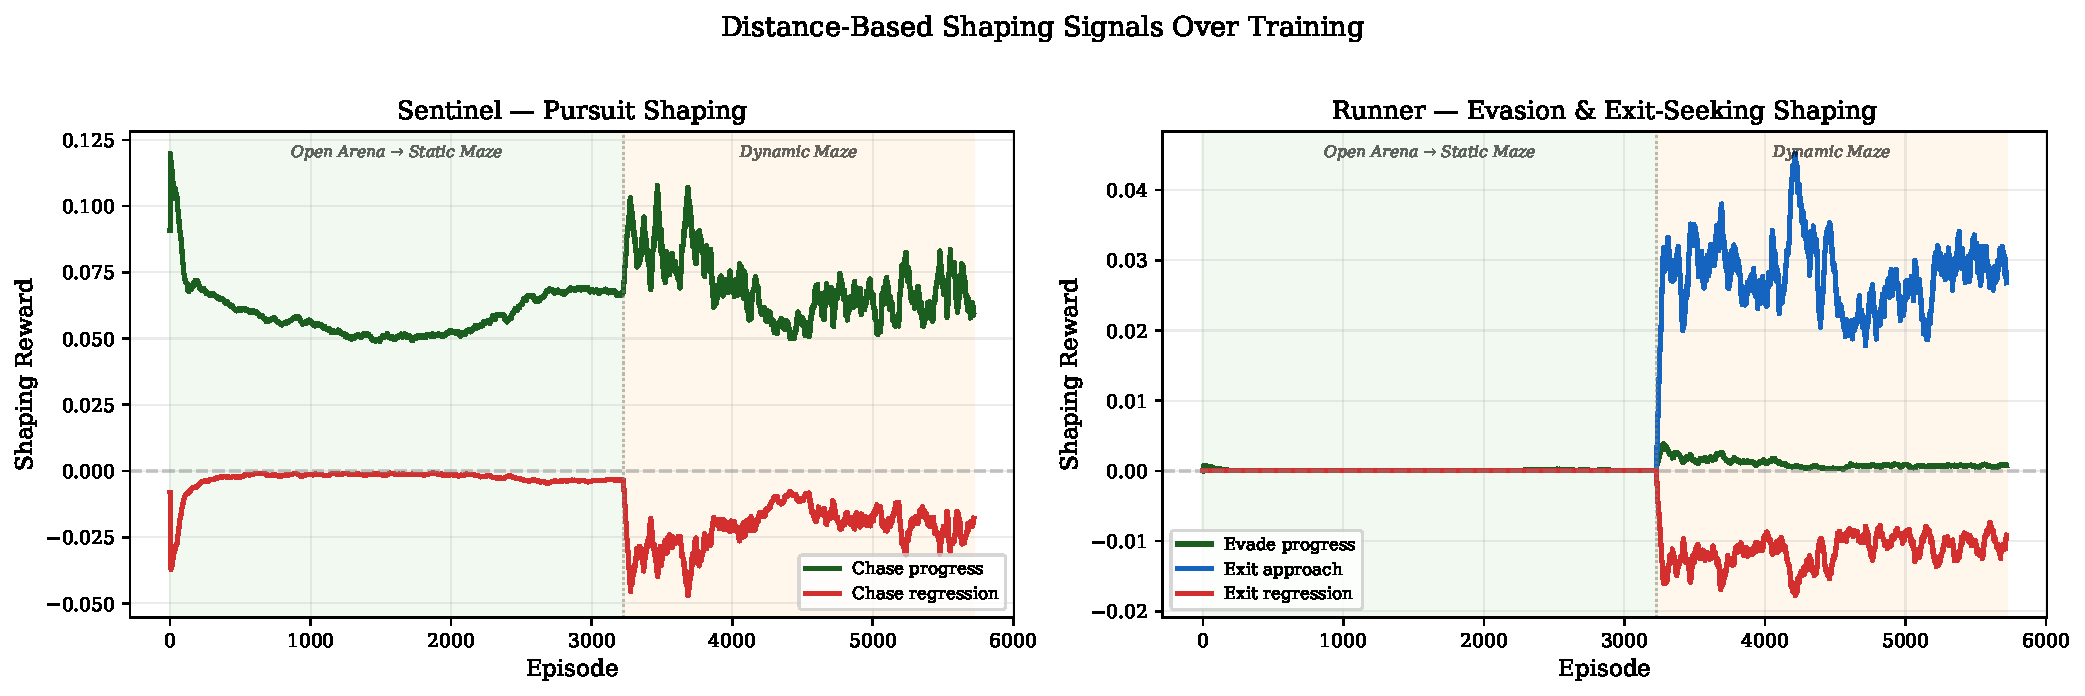
\includegraphics[width=0.48\textwidth]{fig_shaping_signals.pdf}
    \caption{Distance-based shaping signals. Sentinel chase progress (left) and Runner exit-seeking behaviour (right) across curriculum phases.}
    \label{fig:shaping}
\end{figure}

\subsection{Per-Phase Summary}

Figure~\ref{fig:phase_summary} presents the per-phase comparison as bar charts. The progression motivates a curriculum-learning hypothesis, but final zero-shot generalization claims require the expanded unseen-layout protocol.

\begin{figure}[t]
    \centering
    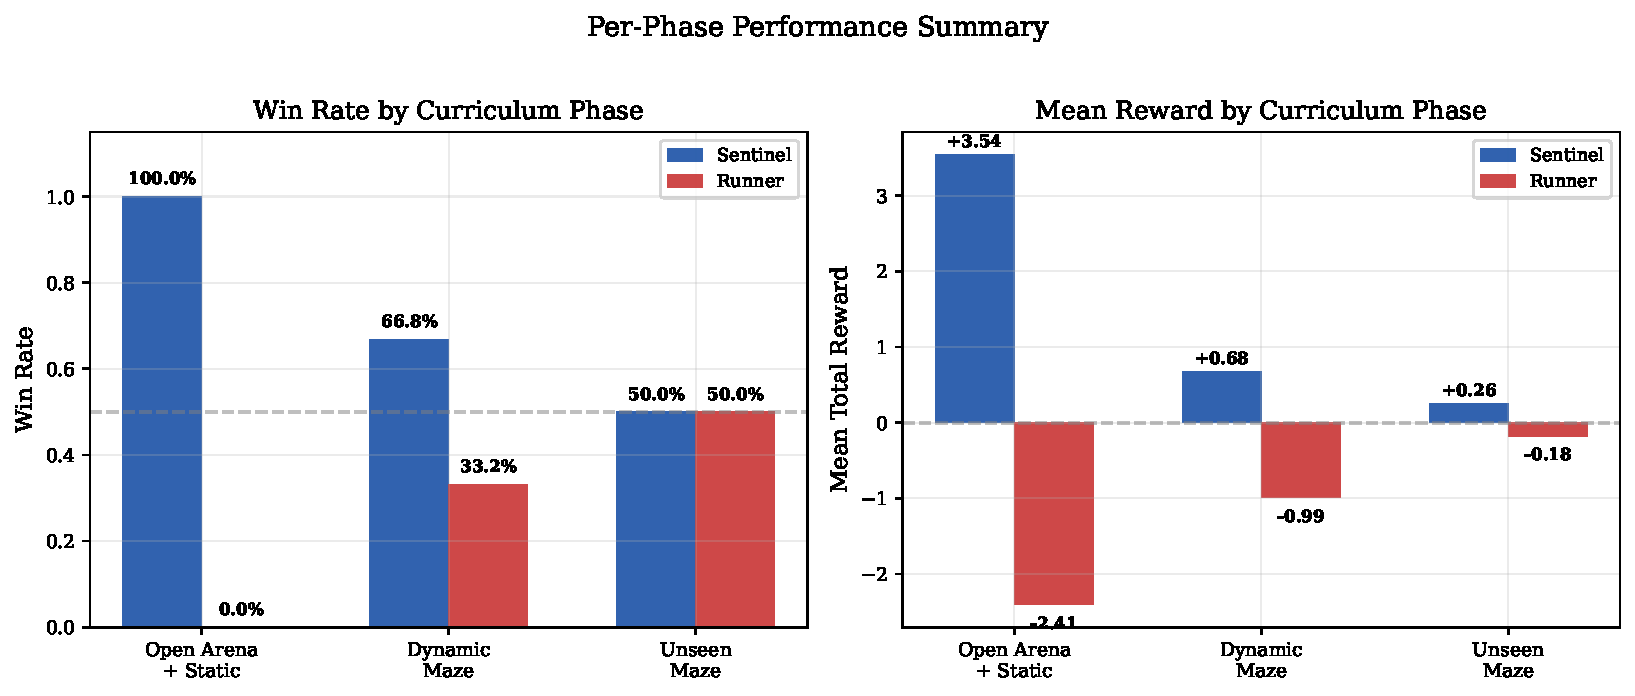
\includegraphics[width=0.48\textwidth]{fig_phase_summary.pdf}
    \caption{Per-phase win rate (left) and mean reward (right). The progressive balancing of win rates motivates the curriculum-learning hypothesis tested by the publication protocol.}
    \label{fig:phase_summary}
\end{figure}

\subsection{Held-Out Configuration Transfer}

The validated diagnostic confirms that the dynamic-maze checkpoint can execute in the held-out scene with seed-specific rule and reward configurations. Across 106 completed unseen-scene episodes, the aggregate Sentinel win rate is 68.9\%. A later code audit established that all five seeds reused one hard-coded topology and that movement/wall parameters differed between seen and unseen files. The 33.3--88.2\% spread is therefore a compound configuration-shift diagnostic, not a topology-generalization result. All cells also use one trained checkpoint pair and short fixed-duration windows. The official experiment must repeat genuinely distinct generated topologies using independently trained policy seeds, matched controls, and fixed episode counts.

% ============================================================
\section{Discussion}
% ============================================================

The results support three main findings.

\textbf{Curriculum learning is a central hypothesis.} The three-phase curriculum with transfer learning appears important for developing complex pursuit-evasion skills. However, this must be verified by a direct-dynamic-training ablation with the same network architecture and evaluation budget.

\textbf{Custom reward shaping targets specific failure modes.} The iterative development of the \texttt{v5\_active\_agents} reward configuration was driven by three observed failure modes:
\begin{itemize}
    \item \textit{Free-rider collapse:} In early training, one Sentinel learned to capture while others remained idle to collect the shared team reward. The \texttt{idle\_penalty} ($-0.002$/step) and increased \texttt{individual\_capture\_bonus} ($+0.25$) were added to reduce this behavior.
    \item \textit{Cluster convergence:} All three Sentinels would chase the same Runner in single file, making evasion trivial. The \texttt{cluster\_penalty} ($-0.015$) encourages spatial separation; publication results must quantify this through Sentinel spread and pincer/corridor metrics.
    \item \textit{Passive evasion:} Runners learned to survive by standing still, avoiding threat-approach penalties but never seeking exits. The \texttt{exit\_approach\_bonus} ($+0.005$) and \texttt{exit\_approach\_regression} ($-0.002$) were added to encourage goal-directed escape behaviour.
\end{itemize}

\textbf{Generalization remains the key empirical test.} The validated fixed-checkpoint diagnostic demonstrates executable transfer to a held-out scene under five configurations, not five topologies. The official protocol tests whether performance and coordination metrics persist across independent policy seeds and genuinely held-out geometries under matched dynamics.

Compared to MatrixWorld~\cite{matrixworld2023}, which provides a grid-based pursuit-evasion benchmark, Labyrinth Breach operates in continuous 3D space with asymmetric teams, dynamic walls, and exit-based objectives. Compared to ViPER~\cite{viper2025}, which focuses on visibility-based pursuit, our environment adds team coordination pressure through the 3v2 asymmetry and tactical reward terms.

% ============================================================
\section{Limitations and Future Work}
% ============================================================

Several limitations remain. First, the current study is simulation-only and does not include physical robot validation. Second, wall collision correctness under all dynamic shift configurations has not been exhaustively validated; rare edge cases during wall transitions could allow agents to clip through geometry. Third, the tactical reward shaping terms add complexity to the reward landscape and could be exploited in ways not yet detected. Fourth, the current architecture uses last-known-position memory rather than recurrent neural memory, which may limit performance in highly dynamic environments. Fifth, the controller includes optional action-assist blending; publication results must disclose it and include an assist-off ablation.

For future work, we plan to: (1) add LSTM memory and compare against the current last-known-position memory; (2) compare PPO with MA-POCA or MAPPO to study centralized credit assignment; (3) complete reward, memory, dynamic-wall, curriculum, and action-assist ablations; and (4) extend the benchmark toward hardware or high-fidelity robot simulators.

% ============================================================
\section{Conclusion}
% ============================================================

We presented Labyrinth Breach, a configurable Unity ML-Agents benchmark for asymmetric multi-agent pursuit-evasion in dynamic mazes. The environment combines dynamic topology, partial observability, exit-directed evasion, and tactical reward shaping in a reproducible 3v2 setting. Preliminary legacy results motivate curriculum learning and reward-shaping hypotheses, but final publication claims require the strict multi-seed evaluation and ablation protocol introduced here. The environment, training configurations, logging pipeline, and trained model checkpoints are publicly available for reproduction and extension.

% ============================================================
\section*{Acknowledgment}
% ============================================================

We acknowledge the AI641 course project brief for defining the original pursuit-evasion direction and motivating the Unity ML-Agents based implementation.

\bibliographystyle{IEEEtran}
\begin{thebibliography}{99}

\bibitem{ai641projectdoc}
AI641 -- AI for Robotics, ``Projects,'' course handout, Project 2: Reinforcement Learning-based multi-agent pursuit-evasion.

\bibitem{lowe2017maddpg}
R. Lowe, Y. Wu, A. Tamar, J. Harb, P. Abbeel, and I. Mordatch,
``Multi-Agent Actor-Critic for Mixed Cooperative-Competitive Environments,''
in \textit{Advances in Neural Information Processing Systems}, 2017.

\bibitem{rashid2018qmix}
T. Rashid, M. Samvelyan, C. S. de Witt, G. Farquhar, J. Foerster, and S. Whiteson,
``QMIX: Monotonic Value Function Factorisation for Deep Multi-Agent Reinforcement Learning,''
in \textit{Proceedings of the 35th International Conference on Machine Learning Workshop}, 2018.

\bibitem{yu2022mappo}
C. Yu et al.,
``The Surprising Effectiveness of PPO in Cooperative Multi-Agent Games,''
in \textit{Advances in Neural Information Processing Systems}, 2022.

\bibitem{verma2019mapel}
T. Verma, F. M. Zegers, and P. P. Khargonekar,
``Multi-Agent Pursuer-Evader Learning using Situation Report,''
arXiv preprint arXiv:1910.07780, 2019.

\bibitem{wang2020implicit}
J. Wang, Y. Ren, T. Yu, H. Zhang, and C. Zhang,
``Learning Implicit Credit Assignment for Cooperative Multi-Agent Reinforcement Learning,''
in \textit{Advances in Neural Information Processing Systems}, 2020.

\bibitem{chen2023explicit}
C. Chen, H. Wang, Y. Hu, and C. Zhang,
``Learning Explicit Credit Assignment for Cooperative Multi-Agent Reinforcement Learning via Polarization Policy Gradient,''
in \textit{Proceedings of the AAAI Conference on Artificial Intelligence}, 2023.

\bibitem{gonultas2024}
O. Gonultas and V. Isler,
``Learning to Play Pursuit-Evasion with Dynamic and Sensor Constraints,''
arXiv preprint arXiv:2405.05372, 2024.

\bibitem{matrixworld2023}
L. Sun, Y.-C. Chang, C. Lyu, C.-T. Lin, and Y. Shi,
``MatrixWorld: A Pursuit-Evasion Platform for Safe Multi-Agent Coordination and Autocurricula,''
arXiv preprint arXiv:2307.14854, 2023.

\bibitem{viper2025}
Y. Wang, Y. Cao, J. Chiun, S. Koley, M. Pham, and G. A. Sartoretti,
``ViPER: Visibility-based Pursuit-Evasion via Reinforcement Learning,''
in \textit{Proceedings of the 8th Conference on Robot Learning}, PMLR, vol. 270, pp. 4188--4200, 2025.

\bibitem{yan2019uncertain}
F. Yan, J. Jiang, K. Di, Y. Jiang, and Z. Hao,
``Multiagent Pursuit-Evasion Problem with the Pursuers Moving at Uncertain Speeds,''
\textit{Journal of Intelligent \& Robotic Systems}, vol. 95, no. 1, pp. 119--135, 2019.

\bibitem{foerster2018coma}
J. Foerster, G. Farquhar, T. Afouras, V. Nardelli, and S. Whiteson,
``Counterfactual Multi-Agent Policy Gradients,''
in \textit{Proceedings of the AAAI Conference on Artificial Intelligence}, 2018.

\bibitem{zhang2023curriculum}
Y. Zhang et al.,
``Curriculum Learning for Cooperation in Multi-Agent Reinforcement Learning,''
in \textit{International Conference on Learning Representations (ICLR) Workshop}, 2023.

\bibitem{li2021teamindividual}
W. Li et al.,
``Team and Individual Rewards for Cooperative Multi-Agent Reinforcement Learning,''
arXiv preprint arXiv:2109.10860, 2021.

\bibitem{liu2024uav}
Y. Liu et al.,
``Multi-UAV Pursuit-Evasion Gaming Based on PSO-M3DDPG Schemes,''
\textit{Complex \& Intelligent Systems}, vol. 10, pp. 5221--5239, 2024.

\bibitem{haeri2022emergent}
H. Haeri, K. Shi, and J. Jeong,
``Emergent Behaviors in Multi-Agent Target Acquisition,''
arXiv preprint arXiv:2212.07891, 2022.

\end{thebibliography}

\end{document}
